\documentclass{article}
\usepackage{graphicx}
\usepackage{enumitem}
\usepackage{hyperref}
\usepackage{listings}
\usepackage{xcolor}
\usepackage{caption}

% Définition des couleurs et du style pour le code
\definecolor{codegray}{gray}{0.9}
\lstdefinestyle{mystyle}{
    backgroundcolor=\color{codegray},
    basicstyle=\ttfamily\small,
    breaklines=true,
    frame=single,
    captionpos=b,
    numbers=left,
    numbersep=5pt,
    numberstyle=\tiny\color{gray},
}
\lstset{style=mystyle}

\title{Document de mi-parcours : Organiz'Asso}
\author{Yuxiang ZHANG \and Antoine LECOMTE}
\date{}

\begin{document}
\maketitle

\section*{Introduction}
Organiz'Asso est une plateforme permettant aux utilisateurs d'échanger des messages et de gérer des discussions. L'architecture repose sur React pour le front-end, avec une organisation en plusieurs composants interconnectés. Ce document décrit les composants clés de notre projet ainsi que leurs dépendances réciproques.

\section*{Graphe des dépendances des composants React}
Le graphe suivant montre les relations entre les composants React du projet, mettant en évidence les dépendances mutuelles et la hiérarchie des composants.

\begin{lstlisting}[caption={Structure des composants React}]
App (index.jsx)
├── MainPage.jsx
│   ├── NavigationPanel.jsx
│   │   ├── Login.jsx
│   │   ├── Logout.jsx
│   │   ├── Signup.jsx
│   ├── Feed.jsx
│   │   ├── SearchBar.jsx
│   │   ├── MessageList.jsx
│   │   │   ├── Message.jsx
│   │   │   │   ├── ReplyList.jsx
│   │   │   │   │   ├── Reply.jsx
│   │   │   │   ├── EditMessage.jsx
│   │   │   │   ├── DeleteMessage.jsx
│   │   ├── AddMessage.jsx
│   ├── UserProfile.jsx
│   │   ├── UserInfo.jsx
│   │   ├── UserSettings.jsx
│   │   ├── UserMessageList.jsx
│   │   │   ├── Message.jsx
│   │   │   │   ├── ReplyList.jsx
│   │   │   │   │   ├── Reply.jsx
│   │   │   │   ├── EditMessage.jsx
│   │   │   │   ├── DeleteMessage.jsx
│   ├── SearchResults.jsx
│   │   ├── MessageList.jsx
│   │   │   ├── Message.jsx
│   │   │   │   ├── ReplyList.jsx
│   │   │   │   │   ├── Reply.jsx
│   │   │   │   ├── EditMessage.jsx
│   │   │   │   ├── DeleteMessage.jsx
│   ├── AdminPanel.jsx
│   │   ├── AdminMenu.jsx
│   │   ├── UserValidation.jsx
│   │   │   ├── ValidateUser.jsx
│   │   ├── AdminFeed.jsx
│   │   │   ├── MessageList.jsx
│   │   │   │   ├── Message.jsx
│   │   │   │   │   ├── ReplyList.jsx
│   │   │   │   │   │   ├── Reply.jsx
│   │   │   │   │   ├── EditMessage.jsx
│   │   │   │   │   ├── DeleteMessage.jsx
│   │   │   ├── AddMessage.jsx
├── api/messagesAPI.jsx
├── api/userAPI.jsx
├── api/serverConfig.jsx
├── context/UserContext.jsx
\end{lstlisting}

\vspace{1cm} % Espacement avant l'image

\begin{figure}[h]
    \centering
    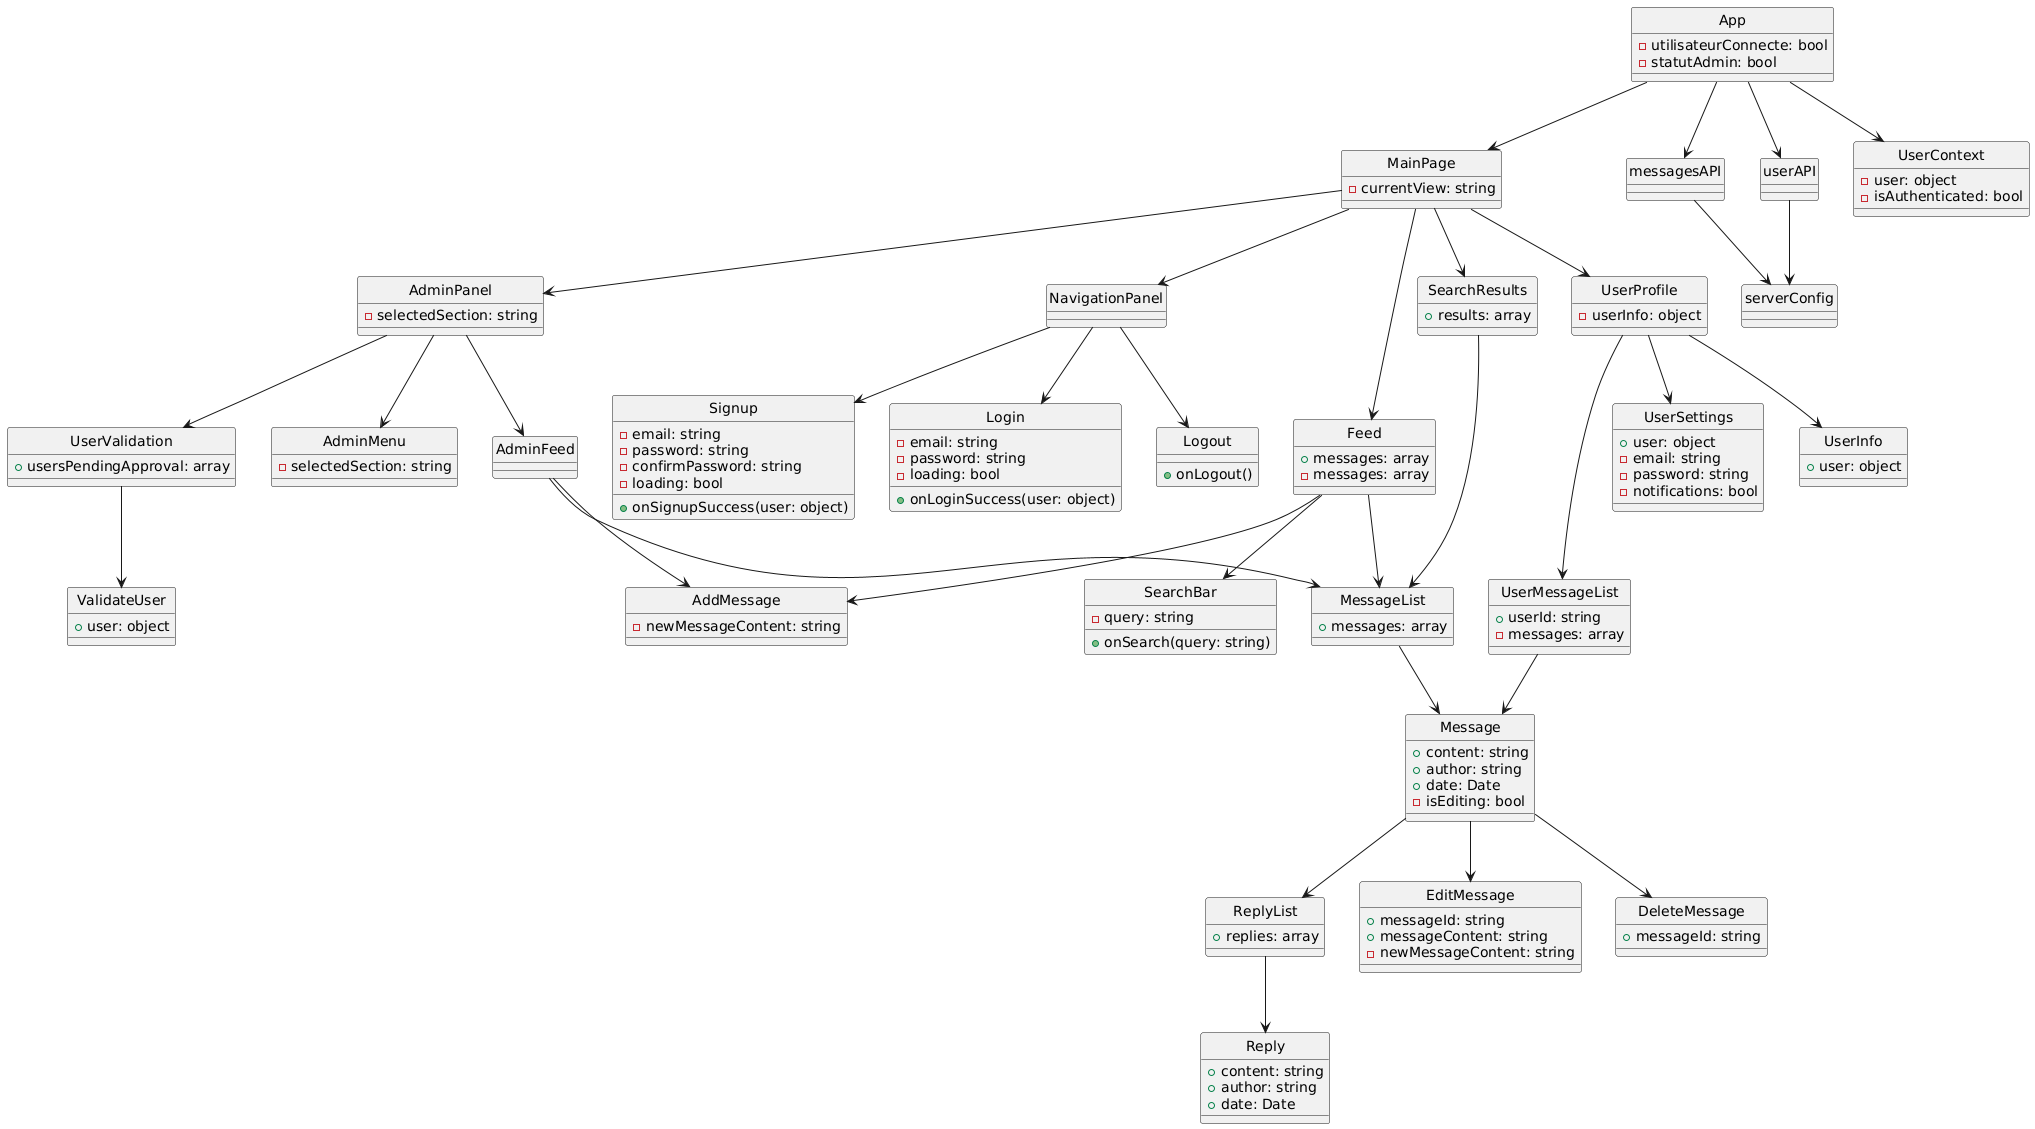
\includegraphics[width=1\linewidth]{Diagramme_uml.png}
    \caption{Diagramme UML des composants}
    \label{fig:uml_diagram}
\end{figure}

\section*{Liste des composants et leur description}

\subsection*{App}
\textbf{Fonction} : Composant principal gérant la navigation et l'état global.\\
\textbf{Props} : Aucune directe.\\
\textbf{State} : Utilisateur connecté, statut administrateur.\\
\textbf{Composants inclus} : MainPage.

\subsection*{MainPage}
\textbf{Fonction} : Page principale affichant la navigation et le contenu central.\\
\textbf{Props} : Aucune directe.\\
\textbf{State} : currentView (string) – Vue actuellement affichée.\\
\textbf{Composants inclus} : NavigationPanel, Feed, UserProfile, SearchResults, AdminPanel.

\subsection*{NavigationPanel}
\textbf{Fonction} : Gère l'authentification des utilisateurs.\\
\textbf{Props} : Aucune.\\
\textbf{State} : Aucun (utilise UserContext).\\
\textbf{Composants inclus} : Login, Logout, Signup.

\subsection*{Login}
\textbf{Fonction} : Permet à un utilisateur de se connecter.\\
\textbf{Props} : onLoginSuccess(user) – Fonction appelée après une connexion réussie.\\
\textbf{State} : email (string), password (string), loading (bool).\\
\textbf{Composants inclus} : Aucun.

\subsection*{Logout}
\textbf{Fonction} : Permet à un utilisateur de se déconnecter.\\
\textbf{Props} : onLogout() – Fonction déclenchée à la déconnexion.\\
\textbf{State} : Aucun.\\
\textbf{Composants inclus} : Aucun.

\subsection*{Signup}
\textbf{Fonction} : Permet à un utilisateur de créer un compte.\\
\textbf{Props} : onSignupSuccess(user) – Fonction appelée après l'inscription.\\
\textbf{State} : email (string), password (string), confirmPassword (string), loading (bool).\\
\textbf{Composants inclus} : Aucun.

\subsection*{Feed}
\textbf{Fonction} : Affiche les messages du forum.\\
\textbf{Props} : messages (array) – Liste des messages.\\
\textbf{State} : Liste des messages.\\
\textbf{Composants inclus} : SearchBar, MessageList, AddMessage.

\subsection*{SearchBar}
\textbf{Fonction} : Permet d’effectuer une recherche dans les messages.\\
\textbf{Props} : onSearch(query) – Fonction appelée lors d’une recherche.\\
\textbf{State} : query (string) – Terme recherché.\\
\textbf{Composants inclus} : Aucun.

\subsection*{MessageList}
\textbf{Fonction} : Liste des messages affichés sur le forum.\\
\textbf{Props} : Liste des messages.\\
\textbf{State} : Aucun.\\
\textbf{Composants inclus} : Message.

\subsection*{Message}
\textbf{Fonction} : Affichage d'un message avec ses réponses.\\
\textbf{Props} : Contenu, auteur, date.\\
\textbf{State} : isEditing (bool) – Indique si le message est en cours d'édition.\\
\textbf{Composants inclus} : ReplyList, EditMessage, DeleteMessage.

\subsection*{ReplyList}
\textbf{Fonction} : Liste des réponses à un message.\\
\textbf{Props} : Liste des réponses.\\
\textbf{State} : Aucun.\\
\textbf{Composants inclus} : Reply.

\subsection*{Reply}
\textbf{Fonction} : Affichage d'une réponse.\\
\textbf{Props} : Contenu, auteur, date.\\
\textbf{State} : Aucun.\\
\textbf{Composants inclus} : Aucun.

\subsection*{EditMessage}
\textbf{Fonction} : Modification d'un message existant dans la discussion.\\
\textbf{Props} : messageId, messageContent.\\
\textbf{State} : newMessageContent.\\
\textbf{Composants inclus} : MessageEditor.

\subsection*{DeleteMessage}
\textbf{Fonction} : Suppression d'un message spécifique de la discussion.\\
\textbf{Props} : messageId.\\
\textbf{State} : Aucun.\\
\textbf{Composants inclus} : Aucun.

\subsection*{AddMessage}
\textbf{Fonction} : Ajout d'un nouveau message dans la discussion.\\
\textbf{Props} : Aucun.\\
\textbf{State} : newMessageContent.\\
\textbf{Composants inclus} : MessageEditor.

\subsection*{UserProfile}
\textbf{Fonction} : Affichage du profil utilisateur.\\
\textbf{Props} : Aucune.\\
\textbf{State} : userInfo (objet) – Informations de l'utilisateur connecté.\\
\textbf{Composants inclus} : UserInfo, UserSettings, UserMessageList.

\subsection*{UserInfo}
\textbf{Fonction} : Affiche les informations d’un utilisateur.\\
\textbf{Props} : user (objet) – Données de l’utilisateur.\\
\textbf{State} : Aucun.\\
\textbf{Composants inclus} : Aucun.

\subsection*{UserSettings}
\textbf{Fonction} : Permet à un utilisateur de modifier ses paramètres (email, mot de passe, préférences).\\
\textbf{Props} : user (objet) – Informations de l’utilisateur actuel.\\
\textbf{State} : email (string), password (string), notifications (bool).\\
\textbf{Composants inclus} : Aucun.

\subsection*{UserMessageList}
\textbf{Fonction} : Affiche les messages publiés par un utilisateur.\\
\textbf{Props} : userId (string) – Identifiant de l’utilisateur.\\
\textbf{State} : messages (array) – Liste des messages.\\
\textbf{Composants inclus} : Message.

\subsection*{SearchResults}
\textbf{Fonction} : Affiche les résultats d’une recherche de messages.\\
\textbf{Props} : results (array) – Liste des messages trouvés.\\
\textbf{State} : Aucun.\\
\textbf{Composants inclus} : MessageList.

\subsection*{AdminPanel}
\textbf{Fonction} : Gère les actions administratives.\\
\textbf{Props} : Aucune.\\
\textbf{State} : selectedSection (string) – Section en cours.\\
\textbf{Composants inclus} : AdminMenu, UserValidation, AdminFeed.

\subsection*{AdminMenu}
\textbf{Fonction} : Menu permettant d’accéder aux outils d’administration.\\
\textbf{Props} : Aucun.\\
\textbf{State} : selectedSection (string) – Section en cours d’affichage.\\
\textbf{Composants inclus} : Aucun.

\subsection*{UserValidation}
\textbf{Fonction} : Gestion des inscriptions et validation des utilisateurs.\\
\textbf{Props} : Liste des utilisateurs en attente.\\
\textbf{State} : Aucun.\\
\textbf{Composants inclus} : ValidateUser.

\subsection*{ValidateUser}
\textbf{Fonction} : Permet d’approuver ou rejeter les utilisateurs en attente.\\
\textbf{Props} : user (objet) – Informations de l’utilisateur à valider.\\
\textbf{State} : Aucun.\\
\textbf{Composants inclus} : Aucun.

\subsection*{AdminFeed}
\textbf{Fonction} : Affichage des discussions du forum privé.\\
\textbf{Props} : Aucun.\\
\textbf{State} : Aucun.\\
\textbf{Composants inclus} : MessageList, AddMessage.

\subsection*{api/messagesAPI}
\textbf{Fonction} : Gestion des requêtes liées aux messages (création, modification, suppression), utilisé dans Feed, MessageList, Message, AddMessage, EditMessage, DeleteMessage, et AdminFeed.\\
\textbf{Props} : Aucun.\\
\textbf{State} : Aucun.\\
\textbf{Composants inclus} : Aucun.

\subsection*{api/userAPI}
\textbf{Fonction} : Gestion des données utilisateur (connexion, déconnexion, récupération des informations utilisateur), utilisé dans Login, Logout, Signup, UserProfile, UserSettings, et UserValidation.\\
\textbf{Props} : Aucun.\\
\textbf{State} : Aucun.\\
\textbf{Composants inclus} : Aucun.

\subsection*{api/serverConfig}
\textbf{Fonction} : Configuration du serveur (paramètres généraux, connexion à la base de données), utilisé par messagesAPI.jsx et userAPI.jsx pour éviter de répéter l’URL de l’API dans chaque requête.\\
\textbf{Props} : Aucun.\\
\textbf{State} : Aucun.\\
\textbf{Composants inclus} : Aucun.

\subsection*{context/UserContext}
\textbf{Fonction} : Fourniture de l'état de l'utilisateur (authentification, informations utilisateur) à travers l'application via le contexte, utilisé dans App.jsx pour gérer l’état global de l’authentification.\\
\textbf{Props} : Aucun.\\
\textbf{State} : user, isAuthenticated.\\
\textbf{Composants inclus} : UserProvider, useUserContext.

\end{document}
